\documentclass[12pt]{article}
\usepackage[utf8]{inputenc}
\usepackage[T1]{fontenc}
\usepackage{titlesec}
\usepackage{listings}
\usepackage{graphicx}
\usepackage{float}
%\usepackage{babel}[it]
% Redefine \ttvar to enable wrapping

\newcommand*\ttvar[1]{\texttt{\expandafter\dottvar\detokenize{#1}\relax}}
\newcommand*\dottvar[1]{\ifx\relax#1\else
  \expandafter\ifx\string.#1\string.\allowbreak\else#1\fi
  \expandafter\dottvar\fi}


\title{Network protocol presentation document\\Peer review \#2}
\author{Berardinelli, Genovese, Grandi, Haddou\\Gruppo AM21}
\date{April 30th, 2024}

\begin{document}

\maketitle


\section{Network protocol}
The network protocol we designed is meant to be implemented with both RMI and Client-Server Socket functionality. Both client and server are equipped with a message parser for serialized Java objects sent through the network and a set of RMI interfaces which are meant to update the views in the client and call controller methods to update the model in the server.

\subsection{Notes on RMI}
In this documentation only \textit{socket} messages are represented, as there is duality in the two approaches since every message corresponds to a remote method invocation.
\newpage
\subsection{General message handling}
\subsubsection{Failed connection handling}
After a connection is enstablished, if the servers fails to respond to a message before the timeout, the clients will try to resend the message for a maximum of 3 times. If the server still fails to respond, the client will close the connection and notify the user that the connection has been lost.
\begin{figure}[H]
    \begin{center}
        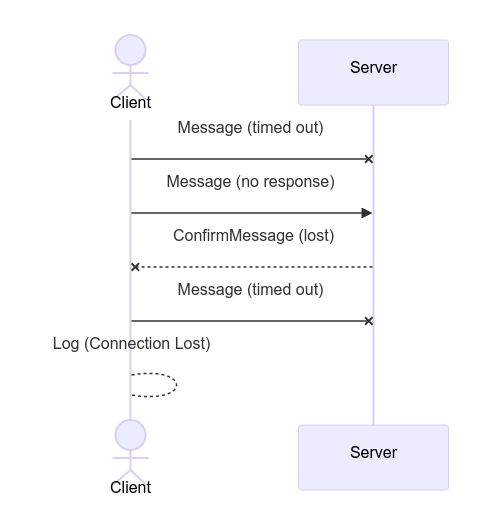
\includegraphics[scale=0.5]{flow_connection.png}
        \caption{Connection Handling}
    \end{center}
\end{figure}

\subsubsection{"Not allowed" message handling}
In the event a client sends a message for an action that the server doesn't expect or that they cannot perform in that moment, and in the event a client might be modified or 'enhanced' in a way the server does not contemplate, we have messages in place to send to the aforesaid client.

\begin{figure}[H]
    \begin{center}
        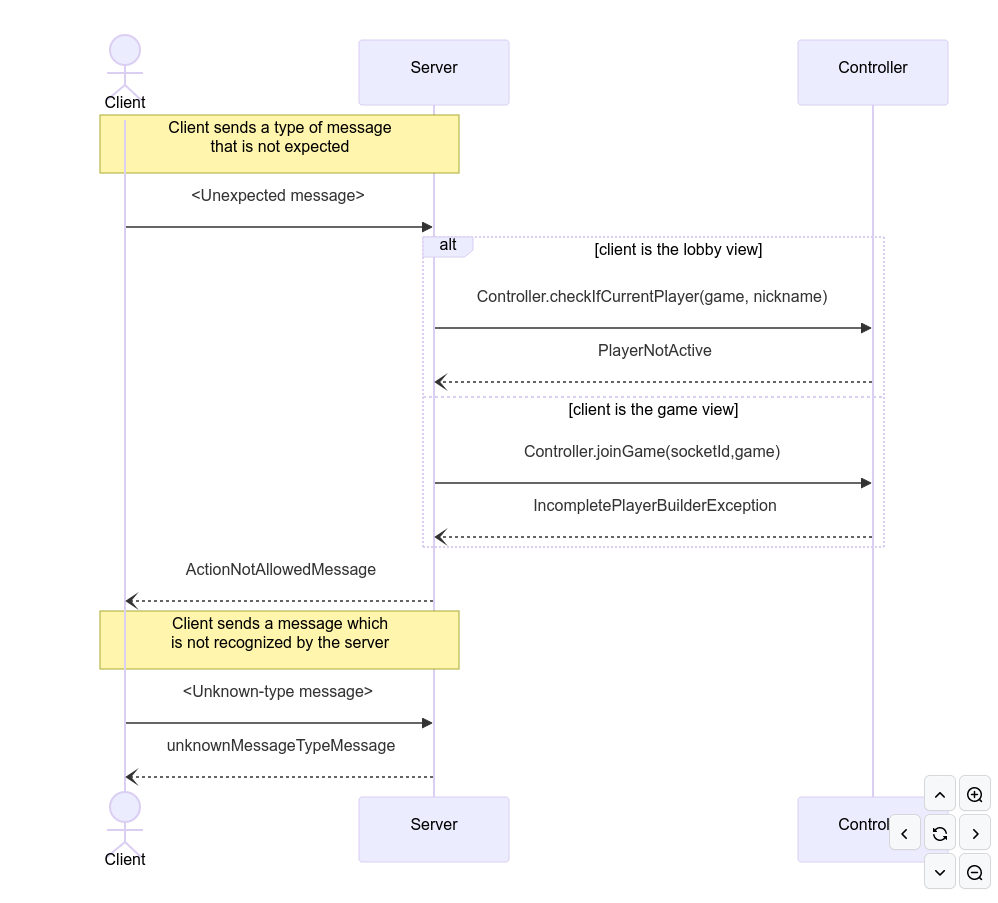
\includegraphics[scale=0.35]{flow_unexpected.png}
        \caption{Connection Handling}
    \end{center}
\end{figure}

\subsection{Game dynamics' flows}
\subsubsection{Lobby flow}
The player building process requires a series of essential steps, which are reported in the following sequence diagram.

Other than \ttvar{ConfirmMessage}, which is required by the client to confirm the message has been received and handled correctly, we added a series of messages whose recipients are all the clients in the lobby or in the game. They are used to update the views of the clients and to notify them of the status of the lobby.

\subsubsection{Normal game turns flow}
Until \ttvar{Game.nextTurn()} detects that a player has a winning score, the messages between the server and the clients are exchanged as follows.

As before, other than the \ttvar{ConfirmMessage}, we have a series of messages whose recipients are all the clients in the game. They are used to update the views of the clients and to notify them of the status of the player turn.
\addtocounter{figure}{2}
\newpage
\subsubsection{Game over flow}
When \ttvar{Game.nextTurn()} detects that a player has a winning score or an \ttvar{EmptyDeckException} is caught by the controller, a message is sent to all the clients to notify them of the number of remaining rounds.

After the final rounds are played, the server will send a series of messages to all the clients to notify them that the game is over and update the final scores of the players after adding the objective cards' points.
\begin{figure}[H]
    \begin{center}
        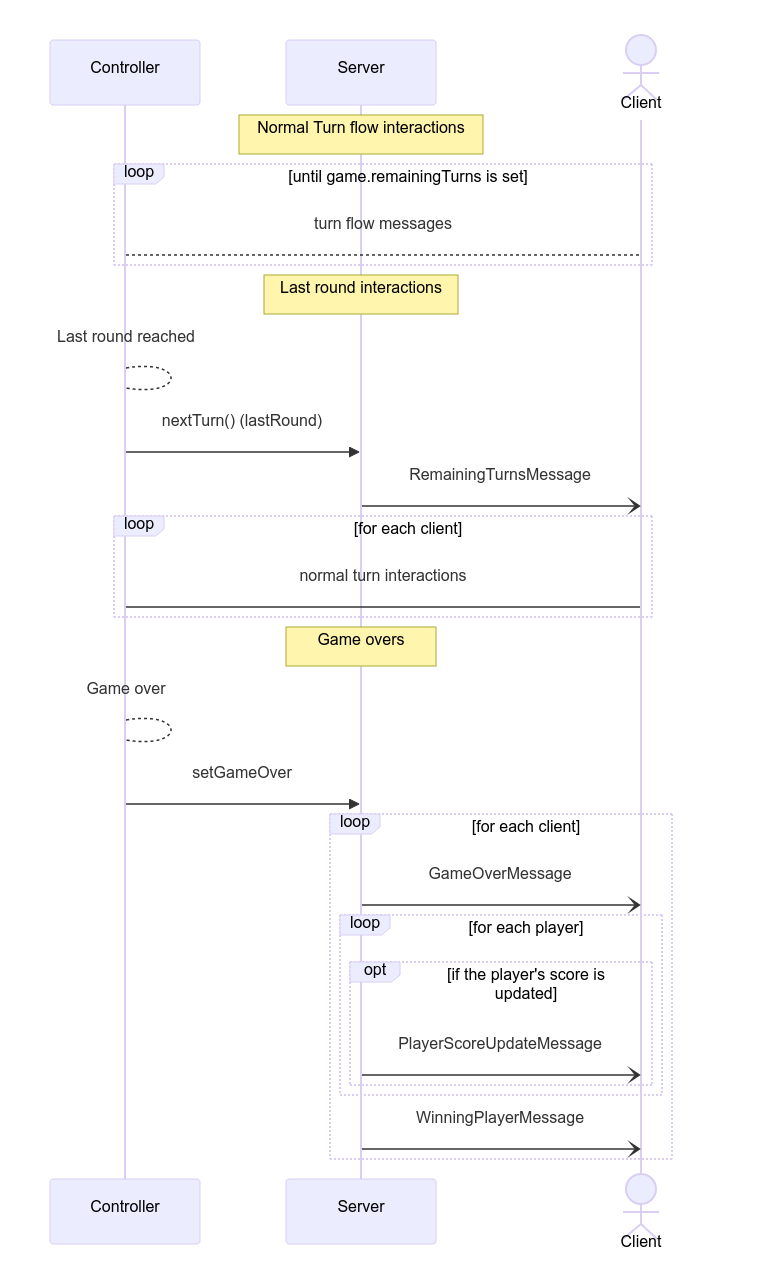
\includegraphics[scale=0.30]{flow_gameover.png}
        \caption{Gameover flow}
    \end{center}
\end{figure}


\subsection{Advanced Features flows}
\subsubsection{Chat}
This exchange happens when a player (Client) wants to write a message in the chat. After PostMessage is sent, the server replies that the message has been received and posted. After that, the server sends a notification to all the recipients of the message informing them that there is a new message in the chat.
\begin{figure}[H]
    \begin{center}
        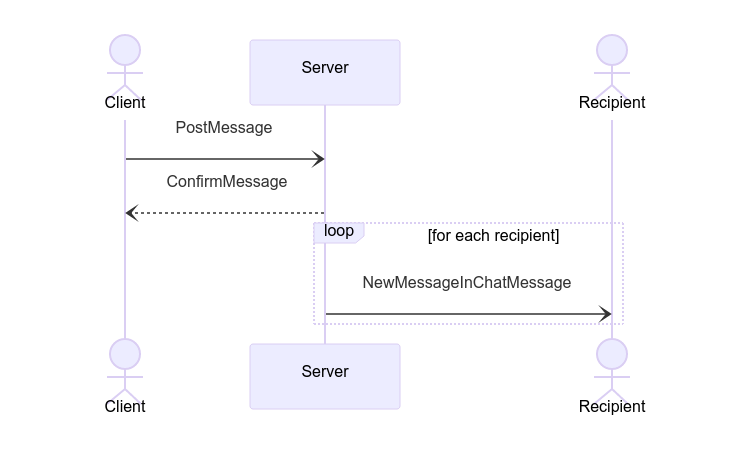
\includegraphics[scale=0.29]{flow_chat.png}
        \caption{Chat flow}
    \end{center}
\end{figure}

\section{Message class structure and uml diagram}
\subsection{Message class structure}
\begin{figure}[H]
    \begin{center}
        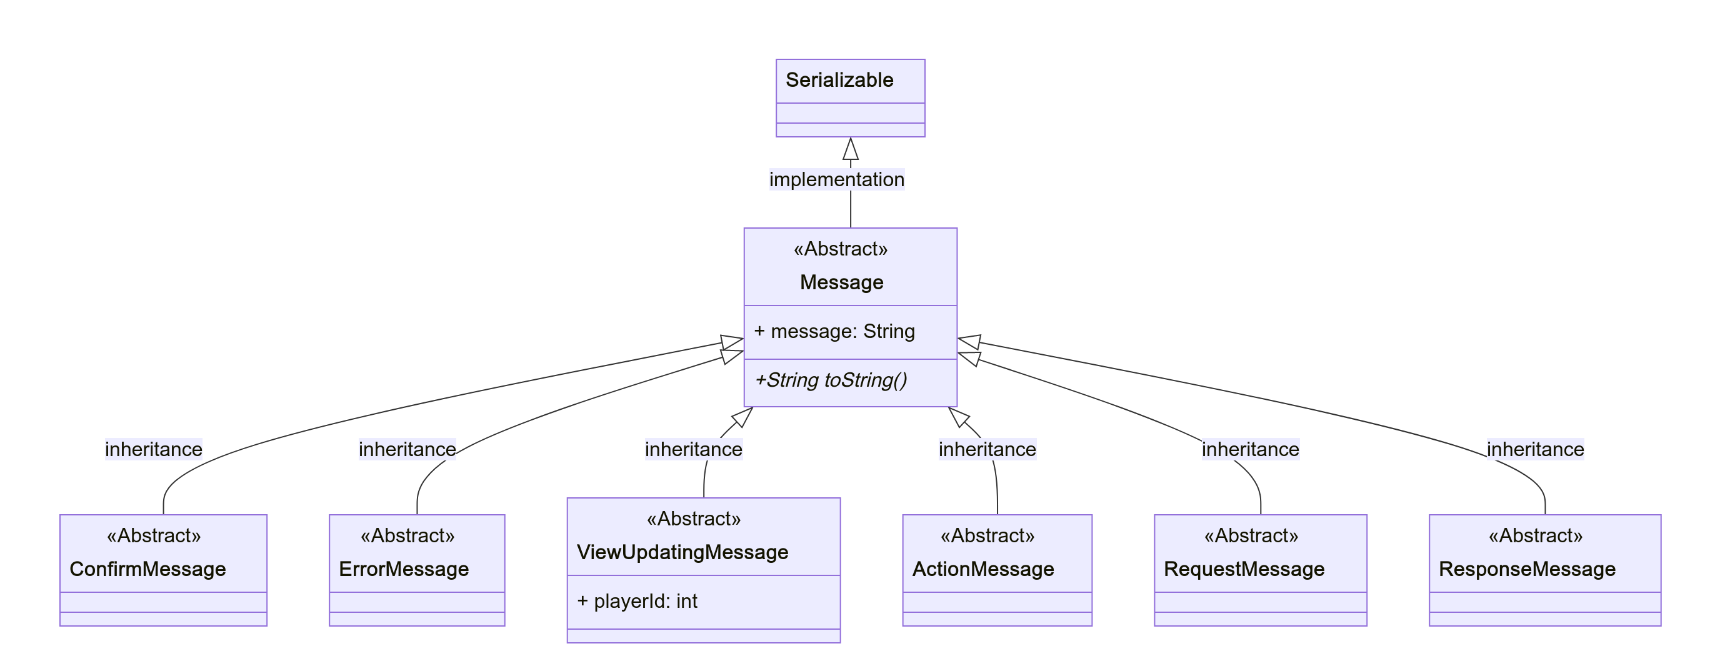
\includegraphics[scale=0.2]{class_diagram_message_class.png}
        \caption{Message abstract class structure and hierarchy} 
    \end{center}
\end{figure}

\subsection{Client requests}
\begin{figure}[H]
    \begin{center}
        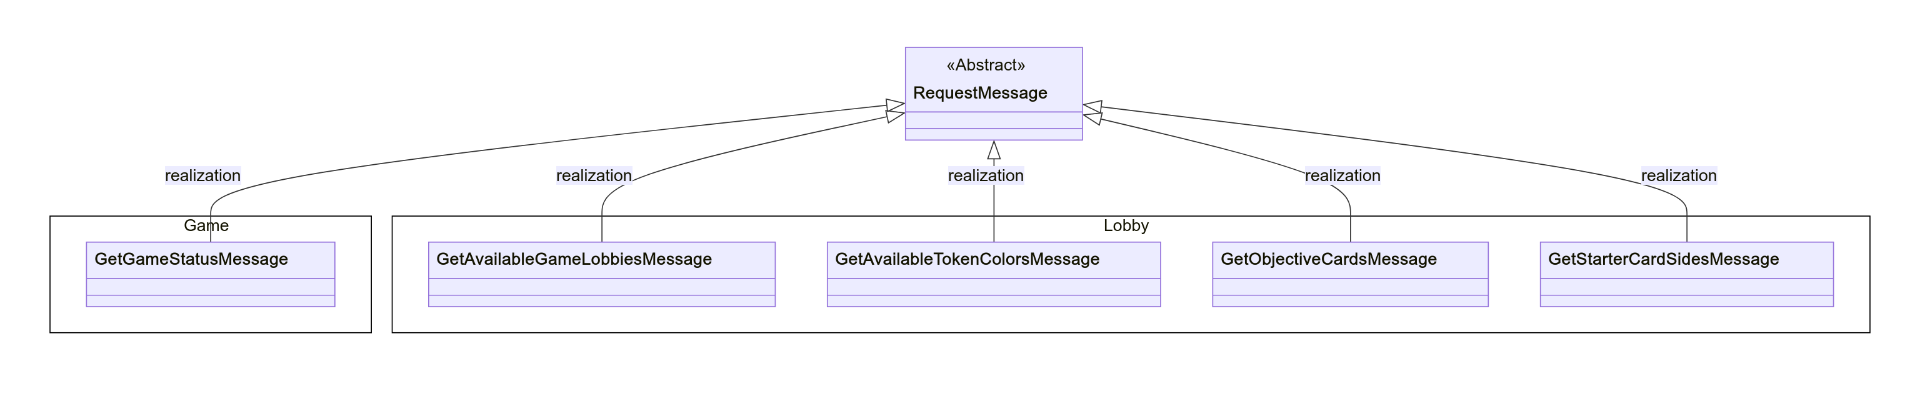
\includegraphics[scale=0.2]{class_diagram_message_client_requests.png}
        \caption{Client requests}
    \end{center}
\end{figure}

\subsection{Server responses}
\begin{figure}[H]
    \begin{center}
        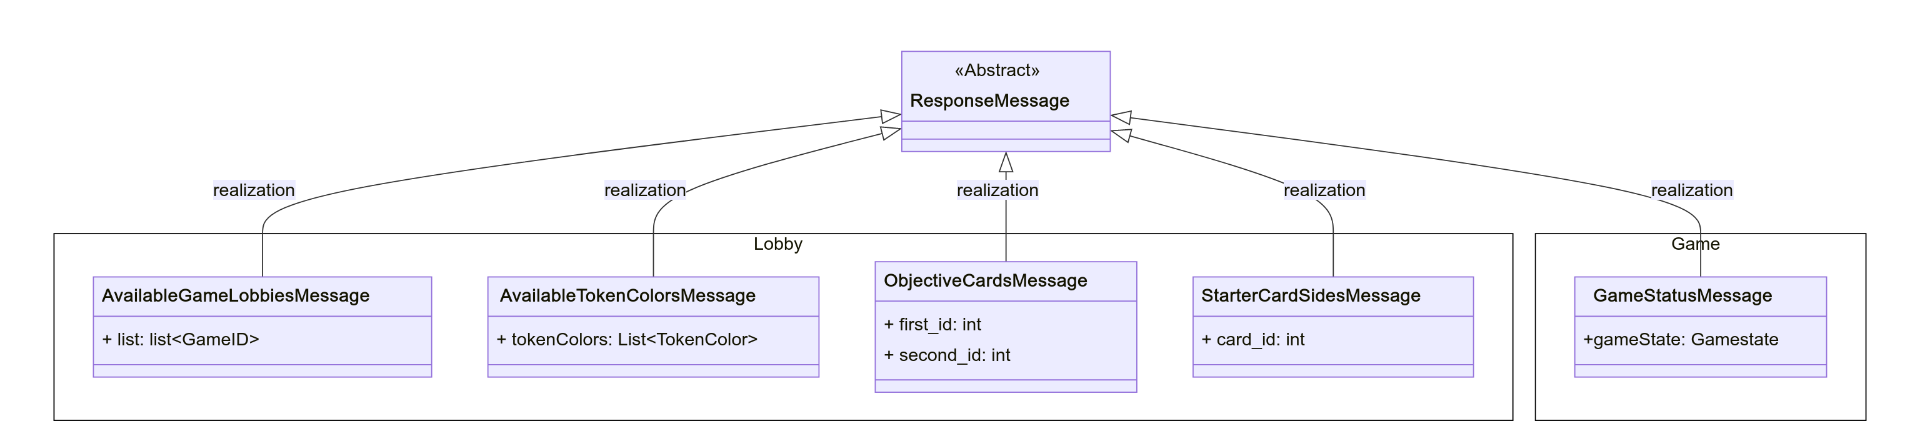
\includegraphics[scale=0.2]{class_diagram_message_server_responses.png}
        \caption{Server responses}
    \end{center}
\end{figure}

\subsection{Client actions}
\begin{figure}[H]
    \begin{center}
        \includegraphics[scale=0.2]{class_diagram_message_client_actions.png}
        \caption{Client actions}
    \end{center}
\end{figure}

\subsection{View updates}
\begin{figure}[H]
    \begin{center}
        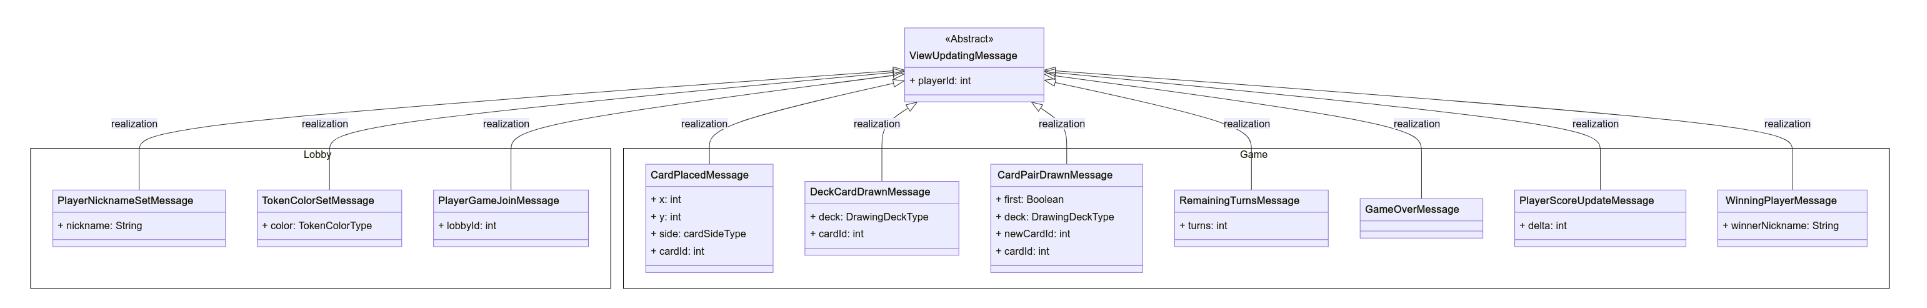
\includegraphics[scale=0.2]{class_diagram_message_viewing_updates.png}
        \caption{View updates}
    \end{center}
\end{figure}

\subsection{Server errors}
\begin{figure}[H]
    \begin{center}
        \includegraphics[scale=0.2]{class_diagram_message_server_errors.png}
        \caption{Server errors}
    \end{center}
\end{figure}

\end{document}
